\chapter{Chain Rule of Partial Differentiation}
\label{chap:chain-rule-of-partial-differentiation}

The chain rule for partial differentiation is a fundamental tool in multivariable calculus that allows us to compute derivatives of composite functions. This chapter explores various forms of the chain rule, from simple cases to more complex scenarios involving multiple variables and intermediate functions.

\section{Chain Rule for Functions with Multiple Variables}
\label{sec:chain-rule-multiple-variables}

\subsection{General Form}

Consider a function \(z = f(x_1, x_2, \ldots, x_n)\) where each variable \(x_i\) is itself a function of \(m\) other variables \(t_1, t_2, \ldots, t_m\). The **chain rule** states that:

\[
  \frac{\partial z}{\partial t_j} = \sum_{i=1}^{n} \frac{\partial f}{\partial x_i} \cdot \frac{\partial x_i}{\partial t_j}
\]

for \(j = 1, 2, \ldots, m\).

\subsection{The 2-2 Case: Two Variables, Two Parameters}

When \(z = f(x, y)\) and both \(x = x(s, t)\) and \(y = y(s, t)\), we have:

\[
  \frac{\partial z}{\partial s} = \frac{\partial f}{\partial x} \cdot \frac{\partial x}{\partial s} + \frac{\partial f}{\partial y} \cdot \frac{\partial y}{\partial s}
\]

\[
  \frac{\partial z}{\partial t} = \frac{\partial f}{\partial x} \cdot \frac{\partial x}{\partial t} + \frac{\partial f}{\partial y} \cdot \frac{\partial y}{\partial t}
\]

\subsubsection{Chain Rule Diamond Trees}

The chain rule can be visualized using **diamond trees** that show the dependency relationships:

\begin{center}
  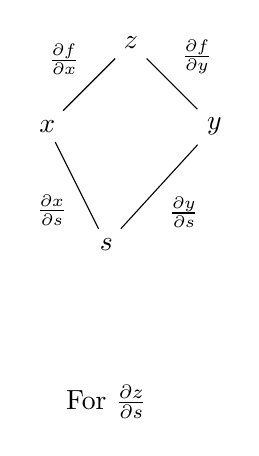
\begin{tikzpicture}[node distance=1.5cm]
    % Tree for ∂z/∂s
    \node (z1) {$z$};
    \node (x1) [below left of=z1] {$x$};
    \node (y1) [below right of=z1] {$y$};
    \node (s1) [below of=x1, xshift=0.75cm] {$s$};

    \draw (z1) -- (x1) node[midway, above left] {\small $\frac{\partial f}{\partial x}$};
    \draw (z1) -- (y1) node[midway, above right] {\small $\frac{\partial f}{\partial y}$};
    \draw (x1) -- (s1) node[midway, below left] {\small $\frac{\partial x}{\partial s}$};
    \draw (y1) -- (s1) node[midway, below right] {\small $\frac{\partial y}{\partial s}$};

    \node [below of=s1, yshift=-0.5cm] {For $\frac{\partial z}{\partial s}$};
  \end{tikzpicture}
  \hspace{2cm}
  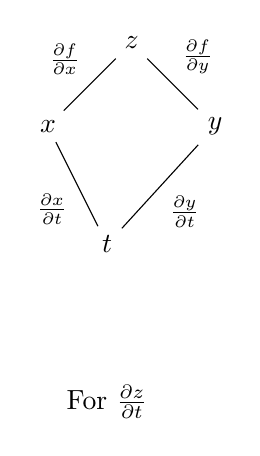
\begin{tikzpicture}[node distance=1.5cm]
    % Tree for ∂z/∂t
    \node (z2) {$z$};
    \node (x2) [below left of=z2] {$x$};
    \node (y2) [below right of=z2] {$y$};
    \node (t2) [below of=x2, xshift=0.75cm] {$t$};

    \draw (z2) -- (x2) node[midway, above left] {\small $\frac{\partial f}{\partial x}$};
    \draw (z2) -- (y2) node[midway, above right] {\small $\frac{\partial f}{\partial y}$};
    \draw (x2) -- (t2) node[midway, below left] {\small $\frac{\partial x}{\partial t}$};
    \draw (y2) -- (t2) node[midway, below right] {\small $\frac{\partial y}{\partial t}$};

    \node [below of=t2, yshift=-0.5cm] {For $\frac{\partial z}{\partial t}$};
  \end{tikzpicture}
\end{center}

\begin{eg}[2-2 Case Example]
  Let \(z = x^2 + y^2\), where \(x = s + t\) and \(y = s - t\). Find \(\frac{\partial z}{\partial s}\) and \(\frac{\partial z}{\partial t}\).

  \textbf{Solution:}
  First, compute the partial derivatives:
  \begin{align}
    \frac{\partial z}{\partial x} &= 2x, \quad \frac{\partial z}{\partial y} = 2y \\
    \frac{\partial x}{\partial s} &= 1, \quad \frac{\partial x}{\partial t} = 1 \\
    \frac{\partial y}{\partial s} &= 1, \quad \frac{\partial y}{\partial t} = -1
  \end{align}

  Using the chain rule:
  \begin{align}
    \frac{\partial z}{\partial s} &= \frac{\partial z}{\partial x} \cdot \frac{\partial x}{\partial s} + \frac{\partial z}{\partial y} \cdot \frac{\partial y}{\partial s} \\
                                  &= 2x \cdot 1 + 2y \cdot 1 = 2(x + y) = 2(2s) = 4s \\
    \frac{\partial z}{\partial t} &= \frac{\partial z}{\partial x} \cdot \frac{\partial x}{\partial t} + \frac{\partial z}{\partial y} \cdot \frac{\partial y}{\partial t} \\
                                  &= 2x \cdot 1 + 2y \cdot (-1) = 2(x - y) = 2(2t) = 4t
  \end{align}
\end{eg}

\subsection{Additional Cases}

\begin{eg}[3-2 Case: Three Variables, Two Parameters]
  Let \(w = f(x, y, z)\) where \(x = x(u, v)\), \(y = y(u, v)\), and \(z = z(u, v)\). Then:
  \[
    \frac{\partial w}{\partial u} = \frac{\partial f}{\partial x} \frac{\partial x}{\partial u} + \frac{\partial f}{\partial y} \frac{\partial y}{\partial u} + \frac{\partial f}{\partial z} \frac{\partial z}{\partial u}
  \]
  \[
    \frac{\partial w}{\partial v} = \frac{\partial f}{\partial x} \frac{\partial x}{\partial v} + \frac{\partial f}{\partial y} \frac{\partial y}{\partial v} + \frac{\partial f}{\partial z} \frac{\partial z}{\partial v}
  \]
\end{eg}

\begin{eg}[3-1 Case: Three Variables, One Parameter]
  If \(w = f(x, y, z)\) where \(x = x(t)\), \(y = y(t)\), and \(z = z(t)\), then:
  \[
    \frac{dw}{dt} = \frac{\partial f}{\partial x} \frac{dx}{dt} + \frac{\partial f}{\partial y} \frac{dy}{dt} + \frac{\partial f}{\partial z} \frac{dz}{dt}
  \]

  \textit{Note:} This is an ordinary derivative since \(w\) depends on only one independent variable \(t\).
\end{eg}

\begin{eg}[2-1 Case: Two Variables, One Parameter]
  For \(z = f(x, y)\) where \(x = x(t)\) and \(y = y(t)\):
  \[
    \frac{dz}{dt} = \frac{\partial f}{\partial x} \frac{dx}{dt} + \frac{\partial f}{\partial y} \frac{dy}{dt}
  \]
\end{eg}

\begin{eg}[3-3 Case: Three Variables, Three Parameters]
  When \(w = f(x, y, z)\) and each variable depends on three parameters \(u\), \(v\), \(s\):
  \[
    \frac{\partial w}{\partial u} = \frac{\partial f}{\partial x} \frac{\partial x}{\partial u} + \frac{\partial f}{\partial y} \frac{\partial y}{\partial u} + \frac{\partial f}{\partial z} \frac{\partial z}{\partial u}
  \]
  with similar expressions for \(\frac{\partial w}{\partial v}\) and \(\frac{\partial w}{\partial s}\).
\end{eg}

\section{Implicit Differentiation}
\label{sec:implicit-differentiation}

When a relationship between variables is given implicitly by an equation \(F(x, y) = 0\), we can find \(\frac{dy}{dx}\) without explicitly solving for \(y\).

\subsection{Theory}

For an equation \(F(x, y) = 0\) that implicitly defines \(y\) as a function of \(x\), the **implicit differentiation formula** is:

\[
  \frac{dy}{dx} = -\frac{\frac{\partial F}{\partial x}}{\frac{\partial F}{\partial y}}
\]

provided that \(\frac{\partial F}{\partial y} \neq 0\).

\textbf{Derivation:} If \(F(x, y) = 0\) and \(y = y(x)\), then by the chain rule:
\[
  \frac{d}{dx}[F(x, y(x))] = \frac{\partial F}{\partial x} + \frac{\partial F}{\partial y} \frac{dy}{dx} = 0
\]

Solving for \(\frac{dy}{dx}\) gives the formula above.

\begin{eg}[Implicit Differentiation Example]
  Find \(\frac{dy}{dx}\) for the circle \(x^2 + y^2 = 25\).

  \textbf{Solution:}
  Let \(F(x, y) = x^2 + y^2 - 25\). Then:
  \begin{align}
    \frac{\partial F}{\partial x} &= 2x \\
    \frac{\partial F}{\partial y} &= 2y
  \end{align}

  Therefore:
  \[
    \frac{dy}{dx} = -\frac{2x}{2y} = -\frac{x}{y}
  \]

  provided \(y \neq 0\).
\end{eg}

\begin{remark}
  Implicit differentiation is particularly useful when solving for \(y\) explicitly would be difficult or impossible, such as with equations like \(xy + \sin(xy) = x^2 + y^3\).
\end{remark}

\section{Directional Derivatives}
\label{sec:directional-derivatives}

The **directional derivative** measures the rate of change of a function in a specific direction, generalizing the concept of partial derivatives.

\subsection{Definition and Derivation}

Let \(f(x, y)\) be a function and \(\mathbf{u} = \langle a, b \rangle\) be a \textbf{unit vector} (i.e., \(|\mathbf{u}| = 1\)). The directional derivative of \(f\) at point \((x_0, y_0)\) in the direction of \(\mathbf{u}\) is defined as:

\subsubsection{Geometric Intuition and Figure}

\begin{center}
  \begin{tikzpicture}[scale=1.2]
    % Draw axes
    \draw[->] (0,0) -- (4,0) node[right] {\(x\)};
    \draw[->] (0,0) -- (0,3) node[above] {\(y\)};

    % Draw the starting point
    \fill (2,1.5) circle (2pt) node[below left=2pt and 2pt] {\(P_o\)};

    % Draw the direction vector
    \draw[->, thick, blue] (2,1.5) -- (2.65,1.85) node[below]{\(\hat{u}\)} ;

    % Draw the point after moving h units
    \fill (3.3,2.2) circle (2pt) node[above=3pt] {\(P\)};

    % Draw the path
    \draw[dashed, red] (2,1.5) -- (3.3,2.2);

    % Add distance label
    \node[red, yshift=5pt] at (2.65,1.85) {\(h\)};

    % Draw level curves with more vertical spacing
    \draw[gray, dashed] (1,0.3) to[bend left=30] (3.6,1.1);
    \draw[gray, dashed] (0.5,1.0) to[bend left=30] (3.9,2.3);
    \draw[gray, dashed] (0.2,2.1) to[bend left=30] (3.5,3.1);

    % Labels for level curves with shifted positions
    \node[gray, font=\small] at (3.7,0.7) {\(f = c_1\)};
    \node[gray, font=\small] at (4.1,2.1) {\(f = c_2\)};
    \node[gray, font=\small] at (3.7,3.2) {\(f = c_3\)};
  \end{tikzpicture}
\end{center}

Let point \(P\) be \((x,y)\).
We know, \(\)
\begin{center}
  \begin{align}
    \vec{P_oP}&=h \hat{u}\\
    \langle x-x_o, y-y_o \rangle &= \langle ha, hb \rangle\\
    \therefore\ \langle x,y \rangle = \langle x_o+ha, y_o+hb \rangle
  \end{align}
\end{center}

Then the differentiation in \(\hat{u}\) direction is given by:
\begin{equation}
  \label{eqn:directional-derivative}
  \begin{displaystyle}
    D_{\mathbf{u}}f(x_0, y_0) = \lim_{h \to 0} \frac{f(x_0 + ha, y_0 + hb) - f(x_0, y_0)}{h}
  \end{displaystyle}
\end{equation}


\subsubsection{Derivation Using the Chain Rule}

\textbf{Step 1: Parameterize the path.}

Let \(g(t) = f(x_0 + ta, y_0 + tb)\). At \(t = 0\), we are at \((x_0, y_0)\), and at \(t = h\), we are at \((x_0 + ha, y_0 + hb)\).

\textbf{Step 2: Recognize the derivative.}

\[
  D_{\mathbf{u}}f(x_0, y_0) = \lim_{h \to 0} \frac{g(h) - g(0)}{h} = g'(0)
\]

\textbf{Step 3: Apply the chain rule.}

Let \(x(t) = x_0 + ta\) and \(y(t) = y_0 + tb\). Then:

\[
  \frac{dx}{dt} = a \quad \text{and} \quad \frac{dy}{dt} = b
\]

By the chain rule:

\[
  g'(t) = \frac{\partial f}{\partial x} \cdot \frac{dx}{dt} + \frac{\partial f}{\partial y} \cdot \frac{dy}{dt} = \frac{\partial f}{\partial x} \cdot a + \frac{\partial f}{\partial y} \cdot b
\]

\textbf{Step 4: Evaluate at the point of interest.}

At \(t = 0\):

\[
  g'(0) = \frac{\partial f}{\partial x}(x_0, y_0) \cdot a + \frac{\partial f}{\partial y}(x_0, y_0) \cdot b
\]

\textbf{Step 5: Express in terms of gradient and dot product.}

The gradient of \(f\) at \((x_0, y_0)\) is:

\[
  \nabla f(x_0, y_0) = \left\langle \frac{\partial f}{\partial x}(x_0, y_0), \frac{\partial f}{\partial y}(x_0, y_0) \right\rangle
\]

Therefore:

\[
  D_{\mathbf{u}}f(x_0, y_0) = \nabla f(x_0, y_0) \cdot \mathbf{u}
\]

\subsubsection{Final Formula}

For a differentiable function \(f(x, y)\) and unit vector \(\mathbf{u} = \langle a, b \rangle\):

\[
  \boxed{D_{\mathbf{u}}f(x_0, y_0) = \nabla f(x_0, y_0) \cdot \mathbf{u} = \frac{\partial f}{\partial x}(x_0, y_0) \cdot a + \frac{\partial f}{\partial y}(x_0, y_0) \cdot b}
\]

\subsubsection{Geometric Interpretation}

The directional derivative \(D_{\mathbf{u}}f(x_0, y_0)\) represents:
\begin{itemize}
  \item The \textbf{slope} of the tangent line to the curve formed by intersecting the surface \(z = f(x, y)\) with a vertical plane containing the direction vector \(\mathbf{u}\)
  \item The \textbf{instantaneous rate of change} of \(f\) per unit distance moved in the direction \(\mathbf{u}\)
\end{itemize}

\subsubsection{Special Cases}

\begin{itemize}
  \item When \(\mathbf{u} = \mathbf{i} = \langle 1, 0 \rangle\): \(D_{\mathbf{i}}f = \frac{\partial f}{\partial x}\)
  \item When \(\mathbf{u} = \mathbf{j} = \langle 0, 1 \rangle\): \(D_{\mathbf{j}}f = \frac{\partial f}{\partial y}\)
\end{itemize}

This shows that partial derivatives are special cases of directional derivatives along the coordinate axes.

\subsection{Computational Formula}

For a differentiable function \(f(x, y)\), the directional derivative can be computed using:

\[
  D_{\mathbf{u}}f(x, y) = \frac{\partial f}{\partial x} a + \frac{\partial f}{\partial y} b = \nabla f \cdot \mathbf{u}
\]

where \(\nabla f = \left\langle \frac{\partial f}{\partial x}, \frac{\partial f}{\partial y} \right\rangle\) is the **gradient** of \(f\).

\subsection{Connection to Partial Derivatives}

\textbf{Special Cases:}
- When \(\mathbf{u} = \mathbf{i} = \langle 1, 0 \rangle\): \(D_{\mathbf{i}}f = \frac{\partial f}{\partial x}\)
- When \(\mathbf{u} = \mathbf{j} = \langle 0, 1 \rangle\): \(D_{\mathbf{j}}f = \frac{\partial f}{\partial y}\)

This shows that **partial derivatives are special cases of directional derivatives** along the coordinate axes.

\begin{eg}[Directional Derivative Example]
  Find the directional derivative of \(f(x, y) = x^2 + xy + y^2\) at point \((1, 2)\) in the direction of vector \(\mathbf{v} = \langle 3, 4 \rangle\).

  \textbf{Solution:}
  First, find the unit vector:
  \[
    |\mathbf{v}| = \sqrt{3^2 + 4^2} = 5 \quad \Rightarrow \quad \mathbf{u} = \left\langle \frac{3}{5}, \frac{4}{5} \right\rangle
  \]

  Compute the partial derivatives:
  \begin{align}
    \frac{\partial f}{\partial x} &= 2x + y \\
    \frac{\partial f}{\partial y} &= x + 2y
  \end{align}

  At point \((1, 2)\):
  \[
    \frac{\partial f}{\partial x}(1, 2) = 4, \quad \frac{\partial f}{\partial y}(1, 2) = 5
  \]

  Therefore:
  \[
    D_{\mathbf{u}}f(1, 2) = 4 \cdot \frac{3}{5} + 5 \cdot \frac{4}{5} = \frac{12}{5} + \frac{20}{5} = \frac{32}{5}
  \]
\end{eg}

\begin{exercise}
  Let \(z = \sin(xy) + x^2y\) where \(x = e^t\) and \(y = t^2\). Find \(\frac{dz}{dt}\) using the chain rule.
\end{exercise}

\begin{answer}
  Using the chain rule:
  \[
    \frac{dz}{dt} = \frac{\partial z}{\partial x} \frac{dx}{dt} + \frac{\partial z}{\partial y} \frac{dy}{dt}
  \]

  Where:
  \begin{align}
    \frac{\partial z}{\partial x} &= y\cos(xy) + 2xy \\
    \frac{\partial z}{\partial y} &= x\cos(xy) + x^2 \\
    \frac{dx}{dt} &= e^t \\
    \frac{dy}{dt} &= 2t
  \end{align}

  Substituting \(x = e^t\) and \(y = t^2\):
  \[
    \frac{dz}{dt} = (t^2\cos(e^t \cdot t^2) + 2e^t \cdot t^2) \cdot e^t + (e^t\cos(e^t \cdot t^2) + e^{2t}) \cdot 2t
  \]
\end{answer}

\begin{remark}
  The chain rule for partial derivatives extends naturally to functions of more variables and more complex dependency structures. The key insight is to trace all possible paths from the dependent variable to the independent variable through the dependency tree, multiplying derivatives along each path and summing the results.
\end{remark}

For more detailed treatments of these topics, see \href{https://tutorial.math.lamar.edu/classes/calciii/chainrule.aspx}{Paul's Online Math Notes} and \href{https://math.libretexts.org/Courses/Monroe_Community_College/MTH_212_Calculus_III/Chapter_13:_Functions_of_Multiple_Variables_and_Partial_Derivatives/13.6:_Directional_Derivatives_and_the_Gradient}{LibreTexts Calculus III}.

